\documentclass[11pt]{amsart}
\usepackage{amsbsy,amsfonts,amsmath,amssymb,amscd,amsthm,mathrsfs,calc,eucal}
\usepackage{graphicx,epsfig,color}
\usepackage{tikz,float}

\begin{document}

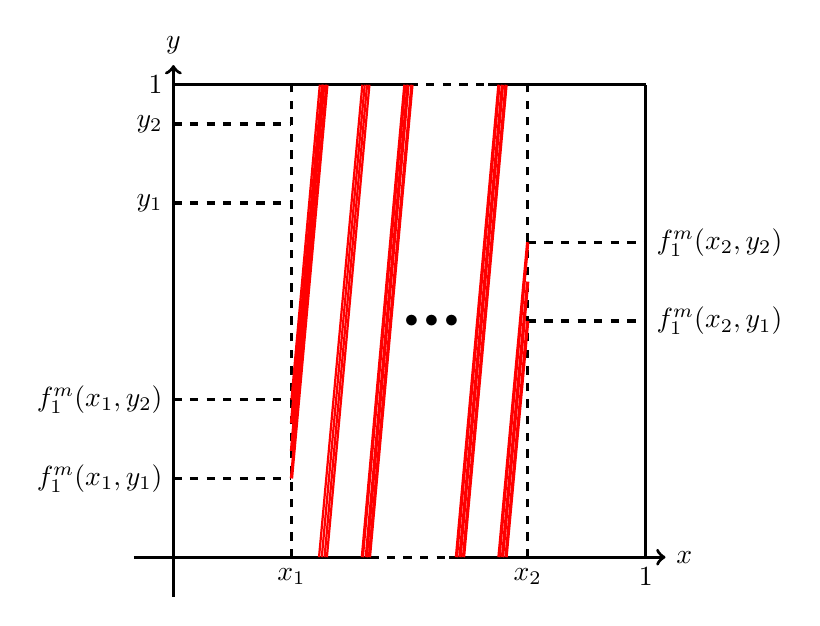
\begin{tikzpicture}[domain=-1:12.5, scale=0.5,very thick]
\draw (-1,0) -- (5,0);
\draw[dashed](5,0)--(7,0);
\draw[->](7,0)--(12.5,0) node[right] {$x$};
\draw[->] (0,-1) -- (0,12.5) node[above] {$y$};
\draw (12,0) -- (12,12);  
\draw[color=black] plot (12,0) node[below] {$1$};
\draw (0,12) -- (6,12);
\draw[dashed](6,12)--(8,12);
\draw(8,12)--(12,12);
\draw[color=black] plot (0,12) node[left] {$1$};




\draw[color=black] plot (3,0) node[below] {$x_1$};
\draw[dashed] (3,0) -- (3,12);

\draw[color=black] plot (9,0) node[below] {$x_2$};
\draw[dashed] (9,0) -- (9,12);

\draw[color=black] plot (0,9) node[left] {$y_1$};
\draw[dashed] (0,9) -- (3,9);

\draw[color=black] plot (0,11) node[left] {$y_2$};
\draw[dashed] (0,11) -- (3,11);




\draw[color=black] plot (0,2) node[left] {$f_1^m(x_1,y_1)$};
\draw[dashed] (0,2) -- (3,2);

\draw[color=black] plot (0,4) node[left] {$f_1^m(x_1,y_2)$};
\draw[dashed] (0,4) -- (3,4);



\draw[color=black] plot (12,6) node[right] {$f_1^m(x_2,y_1)$};
\draw[dashed] (9,6) -- (12,6);

\draw[color=black] plot (12,8) node[right] {$f_1^m(x_2,y_2)$};
\draw[dashed] (9,8) -- (12,8);

\draw[color=red][thick] (3,4) -- (3.72,12);
\draw[color=red] (3,3.4) -- (3.79,12);
\draw[color=red] (3,2.7) -- (3.82,12);
\draw[color=red] (3,2) -- (3.9,12);

\draw[color=red][thick](3.7,0)-- (4.8,12);
\draw[color=red][thick](3.77,0)-- (4.86,12);
\draw[color=red][thick](3.84,0)-- (4.92,12);
\draw[color=red][thick](3.9,0)--(4.98,12);


\draw[color=red](4.8,0)-- (5.88,12);
\draw[color=red](4.9,0)-- (5.96,12);
\draw[color=red](4.98,0)--(6.06,12);


%^^^^^^^^^^^^^^^^^^^^^^^^^^^^^^^^^^^^^^^^^^^^^^^^^^^^^^
\draw[color=black] plot (5.6,6) node[right] {$\bullet\bullet\bullet$};
\draw[color=red](9,6)-- (8.45,0);
\draw[color=red](9,7)-- (8.36,0);
\draw[color=red](9,8)--(8.27,0);


\draw[color=red](7.37,0)-- (8.45,12);
\draw[color=red](7.28,0)-- (8.36,12);
\draw[color=red](7.19,0)--(8.27,12);

\end{tikzpicture}

\end{document}